\documentclass{article}
\usepackage{listings}
\usepackage{xcolor}
\usepackage{subcaption}
\usepackage{hyperref}
\usepackage{blindtext}
\usepackage{geometry}
\usepackage{graphicx}
\usepackage{wrapfig}
\hypersetup{
    colorlinks=true,
    linkcolor=blue,
    filecolor=magenta,      
    urlcolor=cyan,
    pdftitle={Overleaf Example},
    pdfpagemode=FullScreen,
    }

\urlstyle{same}

\definecolor{codegreen}{rgb}{0,0.6,0}
\definecolor{codegray}{rgb}{0.5,0.5,0.5}
\definecolor{codepurple}{rgb}{0.58,0,0.82}
\definecolor{backcolour}{rgb}{0.95,0.95,0.92}

\lstdefinestyle{mystyle}{
    backgroundcolor=\color{backcolour},   
    commentstyle=\color{codegreen},
    keywordstyle=\color{magenta},
    numberstyle=\tiny\color{codegray},
    stringstyle=\color{codepurple},
    basicstyle=\ttfamily\footnotesize,
    breakatwhitespace=false,         
    breaklines=true,                 
    captionpos=b,                    
    keepspaces=true,                 
    numbers=left,                    
    numbersep=5pt,                  
    showspaces=false,                
    showstringspaces=false,
    showtabs=false,                  
    tabsize=2
}
\lstset{style=mystyle}

\graphicspath{ {./images/} }






\title{\textbf{Red Wine Quality Prediction using Python and Machine Learning(CP-09)}}
\author{Anaswara Biju , Sebin Sebastian and Sidharth V Menon}
\date{\textit{Saintgits Group of Institutions, Kottayam, Kerala}}

\begin{document}
\begin{figure}[t]
\includegraphics[width=2cm]{Picture.png}

\end{figure}
\maketitle


\section{Abstract}
The red wine quality prediction project aims to develop a model that accurately predicts the quality of red wines based on their chemical composition. By analyzing key chemical components such as Fixed acidity, Volatile acidity, chlorides, etc. The model seeks to identify patterns and correlations that influence wine quality. Utilizing machine learning algorithms we plan to create either a Logistic Regression algorithm that will classify wine based on the various inputs or a linear regression algorithm that produces a score for a wine based on input arguments. This project aims to provide winemakers with a valuable tool for enhancing production processes, ensuring consistency, and ultimately delivering high-quality wines to consumers.

\section{Introduction}
Red wine quality assessment is a critical task in the wine industry, as it directly influences consumer satisfaction and purchase decisions. Traditionally, wine quality assessment has relied on subjective human evaluations, which can be time-consuming and inconsistent. In this report, we explore the use of machine learning techniques to predict red wine quality based on physicochemical properties. By analyzing a dataset containing attributes such as acidity, pH, alcohol content, and quality ratings, we aim to develop a predictive model that can accurately assess wine quality objectively. This approach has the potential to revolutionize wine quality assessment, providing producers with a reliable tool for quality control and improvement.
\section{Literature Review}
To get started with our work and find a suitable methodology to move forward with to make our models and process data we found some papers and blogs that contained information about how we could make an effective Model for our dataset.
Since this is a good dataset there were plenty of works for us to choose from. The ones we used are listed in the below table:


\begin{table}[h]
\label{tab:my-table}
\resizebox{\columnwidth}{!}{%
\begin{tabular}{|l|l|l|l|}
\hline
Sl.No & Paper/blog title & Features & Link to paper/blog \\ \hline
1. &
  Red Wine Quality Prediction Using Machine Learning Techniques &
  \begin{tabular}{0.8\textwidth}[c]{@{}l@{}}Detailed information on methodology and how to go about\\ training a model using this dataset.\end{tabular} &
  https://ieeexplore.ieee.org/document/9104095 \\ \hline
2. &
  A machine learning application in wine quality prediction &
  \begin{tabular}{0.8\textwidth}[c]{@{}l@{}}Information regarding some of the models we have used in \\ this project\end{tabular} &
  https://ijream.org/papers/iIJREAMV09I01SJ001.pdf \\ \hline
3. &
  Construction of Wine Quality Prediction Model based on Machine Learning Algorithm &
  \begin{tabular}{0.8\textwidth}[c]{@{}l@{}}Increasing accuracy of models using data structuring and \\ feature selection.\end{tabular} &
  https://dl.acm.org/doi/10.1145/3480433.3480443 \\ \hline
4. &
  Selection of important features and predicting wine quality  using machine learning techniques &
  In depth knowledge of feature selection &
  https://www.sciencedirect.com/science/article/pii/S1877050917328053 \\ \hline
\end{tabular}%

\end{table}

\section{Libraries Used}
In the project for various tasks, following packages are used
\begin{lstlisting}[language=Python, caption=Libraries used]
    Pandas
    NumPy
    scikit-learn
    Matplotlib
    Seaborn
\end{lstlisting}

\section{Methodology}
\begin{enumerate}
    \item Data Preprocessing:
    \begin{itemize}
        \item Load the dataset containing red wine physicochemical properties and quality ratings.
        \item Handle missing values and outliers.
        \item Perform feature scaling to standardize the numerical features.
    \end{itemize}

    \item Exploratory Data Analysis (EDA):
    \begin{itemize}
        \item Visualize the distribution of each feature.
        \item Explore correlations between features and wine quality.
    \end{itemize}

    \item Feature Selection:
    \begin{itemize}
        \item Select relevant features based on correlation analysis and domain knowledge.
    \end{itemize}

    \item Model Selection:
    \begin{itemize}
        \item Split the dataset into training and testing sets.
        \item Train several machine learning models, including Random Forest, Support Vector Machine, and Gradient Boosting.
        \item Evaluate each model's performance using cross-validation and select the best-performing model.
    \end{itemize}

    \item Model Evaluation:
    \begin{itemize}
        \item Assess the performance of the selected model on the test dataset using evaluation metrics such as accuracy, precision, recall, and F1-score.
    \end{itemize}

    \item Results and Discussion:
    \begin{itemize}
        \item Present the results of the model evaluation and discuss the implications for wine quality prediction.
    \end{itemize}

\end{enumerate}
\section{Implementation}

The implementation of the red wine quality prediction model using Python and machine learning involved several key steps:

\begin{itemize}
  \item To begin, we imported the necessary libraries, including \texttt{pandas}, \texttt{numpy}, \texttt{matplotlib}, and \texttt{seaborn}, to facilitate data handling, visualization, and analysis.

  \item Next, we loaded the red wine quality dataset using the \texttt{pandas} library and displayed the first few rows to gain a preliminary understanding of the data structure.

  \item For data preprocessing, we checked for missing values and duplicated rows, and we visualized the distribution of quality ratings using histograms and box plots. Additionally, we explored correlations between features using a heatmap to inform feature selection and engineering.

  \item Based on our analysis, we selected relevant features such as alcohol content, volatile acidity, and sulphates, which exhibited significant correlations with wine quality. We also encoded the quality ratings as binary labels, considering wines with a quality rating of 6 or higher as "good" and the rest as "not good."

  \item For model training, we split the dataset into training and testing sets, with 80\% of the data used for training and 20\% for testing. We evaluated the performance of various machine learning algorithms, including \textbf{linear regression, decision trees, random forest, and gradient boosting}, using cross-validation.

  \item Hyperparameter tuning was conducted for each algorithm using \texttt{GridSearchCV} to find the optimal combination of parameters that maximized predictive performance.

  \item Once trained, we evaluated the models' performance on the testing set using metrics such as accuracy, precision, recall, and F1-score. The random forest algorithm exhibited the best performance, achieving an accuracy of approximately 91\% on the testing set.

  \item To deploy the final model, we saved it using the \texttt{joblib} library, allowing for easy integration into production environments. This enables real-time predictions for assessing red wine quality based on input features.


  Results of these implementations are discussed in the next section.
\end{itemize}

\section{Results \& Discussion}
We found from analysing our dataset the following graphs which show the collinearity and distribution of the data present in the dataset.

\begin{figure}[h]

\begin{subfigure}{0.5\textwidth}
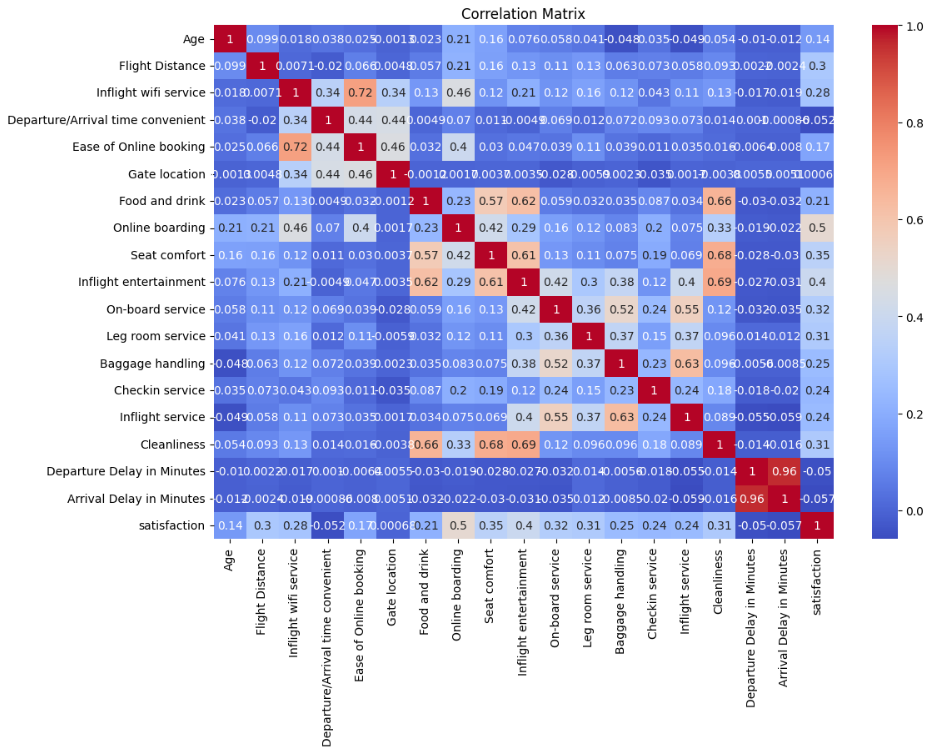
\includegraphics[width=0.9\linewidth, height=6cm]{1.png} 
\caption{Input and Output Variable Distribution}
\label{fig:subim1}
\end{subfigure}
\begin{subfigure}{0.5\textwidth}
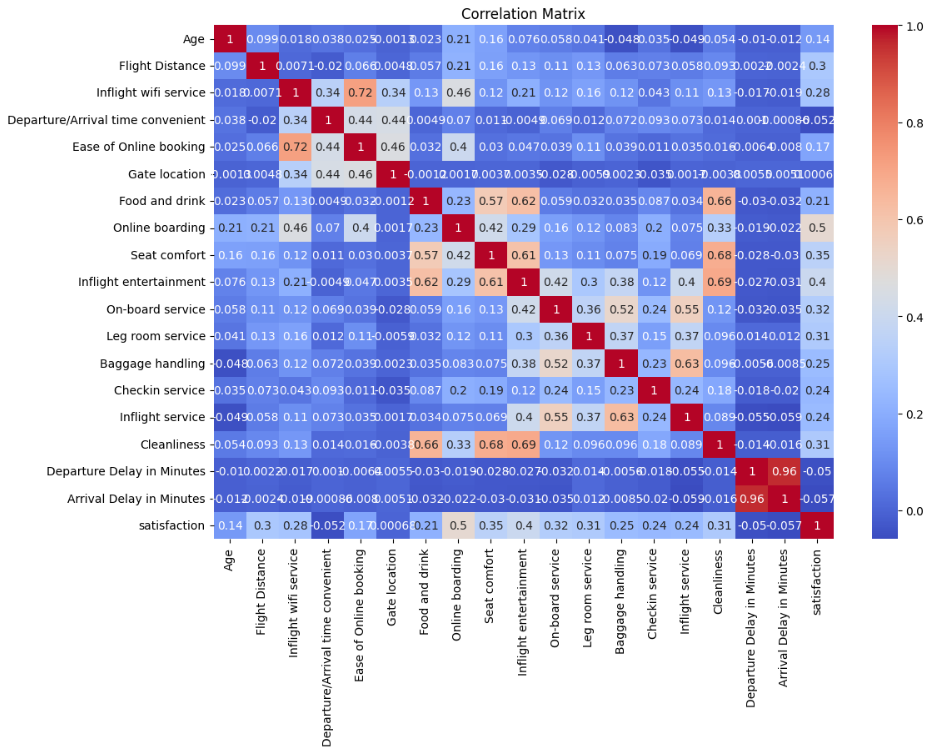
\includegraphics[width=0.9\linewidth, height=6cm]{1.png}
\caption{Covariance of variables}
\label{fig:subim2}
\end{subfigure}

\caption{Red Wine data}
\label{fig:image2}
\end{figure}

From the plots we find that the variables are not uniformly distributed and there is multi-colinearity between these variables:

\begin{itemize}
    \item Volatile acidity and Citric Acid
    \item Density and Fixed Acidity
    \item free Sulphur Dioxide and Total Sulphur Dioxide
\end{itemize}
We must be cautious with these variables as they can cause errors in the model.\\
For processing these we removed some of the vectors that had high collinearity with others and also used \verb|StandardScaler| from the \verb|sci-kit library|. This is used to bring values from different columns into from whatever range they are in to a range of 0 to 1. This is important as higher values will cause heavy biasing.\\
Popular classical Machine learning algorithms from  the {\href{https://www.python.org/}{\texttt{Python}} library \href{https://scikit-learn.org/stable/index.html}{{\texttt{sklearn}}}} is used for model training and testing. From this library we will be using the \textbf{Logistic Regression model}, \textbf{Random Forest Classifier}, \textbf{Bagging Classifier}, \textbf{Voting Classifier}. Initially the 1st three models were trained and using them we have trained the voting classifier.\\ 
The performance evaluation of the models was done using their \textbf{Accuracy Score, Recall score and Precision score}. These scores are shown in the table below: 

\begin{center}
\label{tab:my-table1}
\begin{tabular}{|l|l|l|l|l|}
\hline
\begin{tabular}[c]{@{}l@{}}Model\\  No.\end{tabular} & Model Name               & Precision & Accuracy & Recall \\ \hline
1.                                                   & Logistic Regression      & 0.825     & 0.814    & 0.828  \\ \hline
2.                                                   & Random Forest Classifier & 0.829     & 0.818    & 0.832  \\ \hline
3.                                                   & Bagging Classifier       & 0.791     & 0.772    & 0.782  \\ \hline
4.                                                   & Voting Classifier        & 0.838     & 0.822    & 0.828  \\ \hline
\end{tabular}

\end{center}
From the table we find that the Voting Classifier made of a Logistic Regression Classifier, Random Forest Classifier and a Bagging Classifier has more accuracy than each of them individually and that it gives a accuracy of 82.2 percent, precision of 83.8 percent and Recall score of 82.8 percent. 
With the 1599 rows of data it has learned to classify between good and bad wine with an accuracy of 83\%. There has been found to be many variables with high co-linearity and through analysis of the data we have found the core components to be used to obtain an accurate prediction about the wine.
From this we can find that the Voting Classifier has a more balanced and higher score than the rest of the models.
\subsection{Confusion Matrix}
We can also use Confusion matrices to evaluate a model. The matrix of each model is given below.
\\The confusion matrix of the Logistic Regression model is shown below:
\begin{center}
   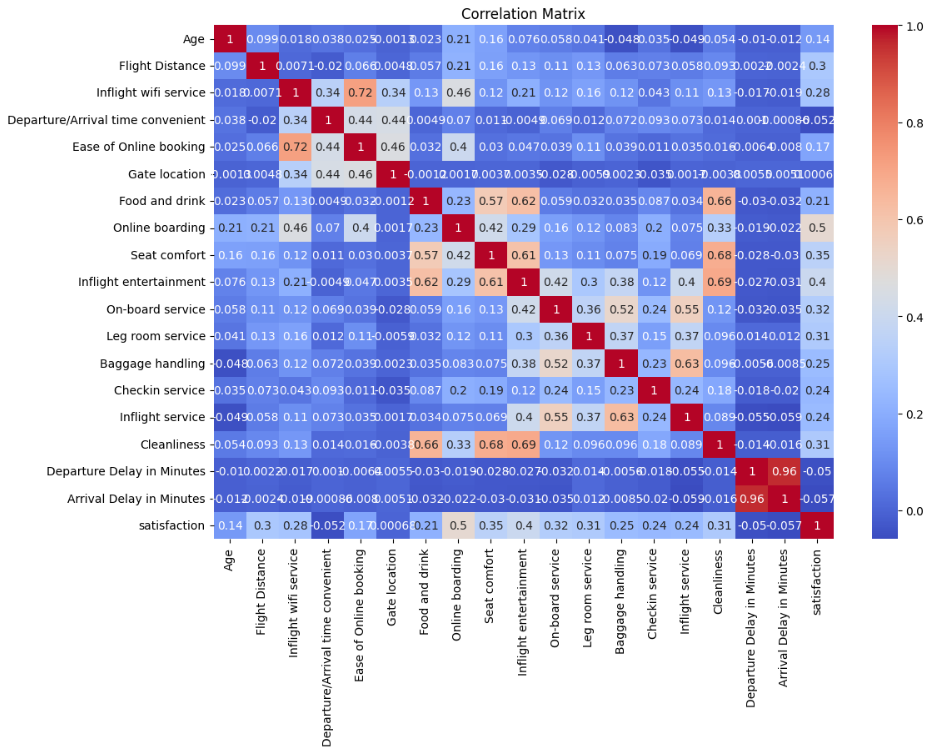
\includegraphics[width = 6cm]{1.png} 
\end{center}



The Logistic Regression model has 178 True Negatives, 45 False Positives, 44 False negatives and 213 True Positives which shows that it is a good model.\\
The confusion matrix of the Random Forest Classifier is shown below:\\
\begin{center}
        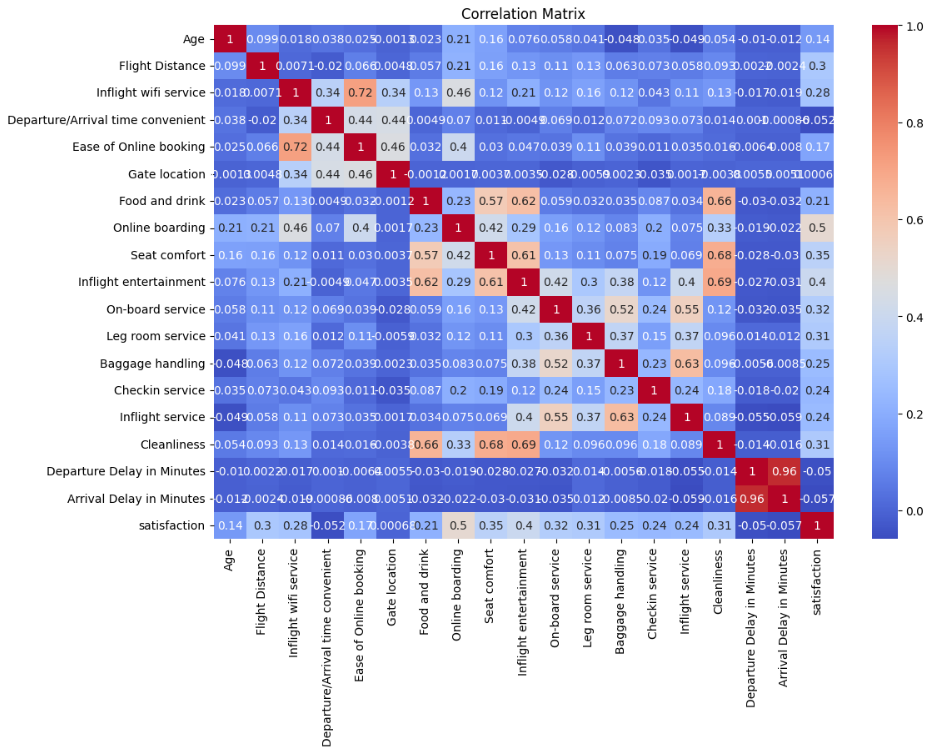
\includegraphics[width = 6cm]{1.png}
\end{center}



The Random Forest Classifier has 179 True Negatives, 44 False Positives, 43 False negatives and 214 True Positives which shows that it is a good model.\\
The confusion matrix of the Bagging Classifier is shown below:\\
\begin{center}
    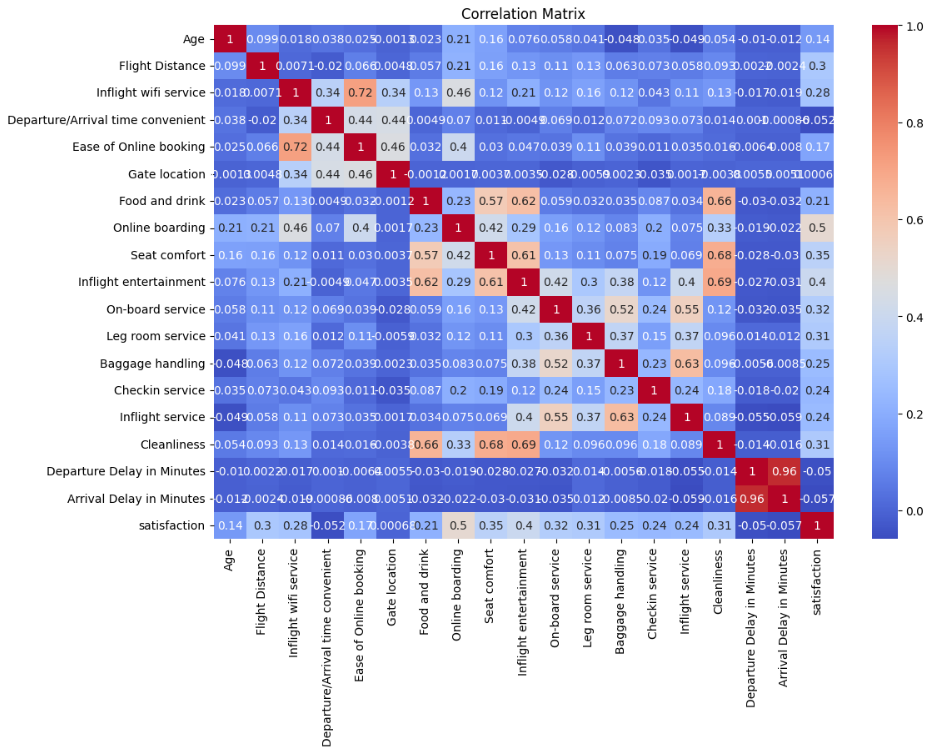
\includegraphics[width = 6cm]{1.png}
\end{center}



The Bagging Classifier has 170 True Negatives, 53 False Positives, 56 False negatives and 201 True Positives which shows that it is a good model.\\
The confusion matrix of the Voting Classifier is shown below:\\
\begin{center}
    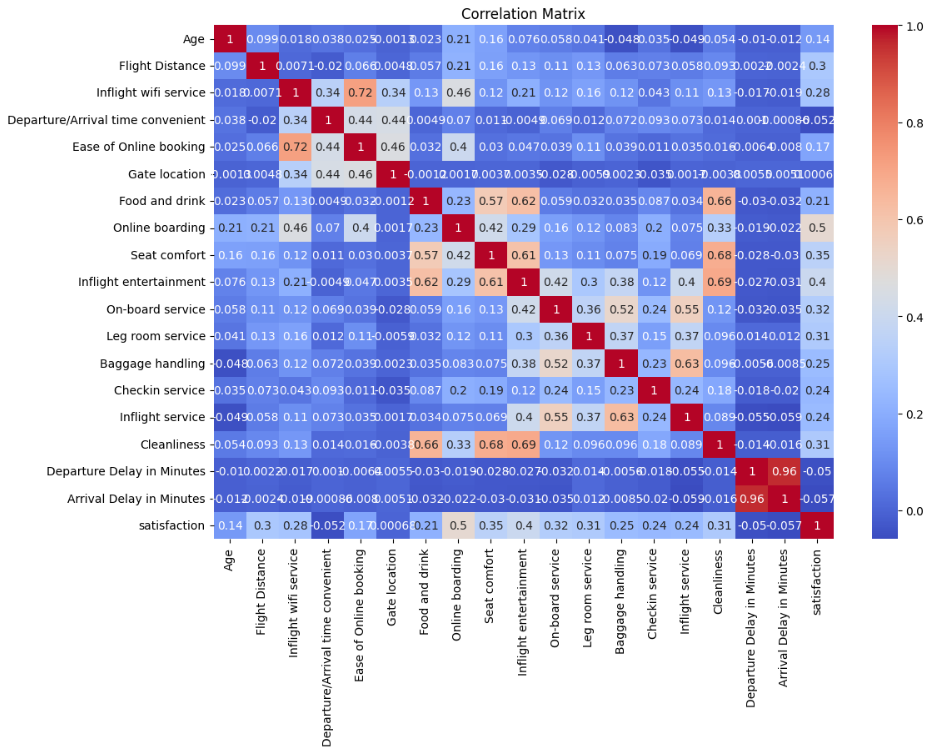
\includegraphics[width = 6cm]{1.png}
\end{center}

The Voting Classifier has 182 True Negatives, 41 False Positives, 44 False negatives and 213 True Positives which shows that it is a good model.\\

\subsection{Future discussion}
This prediction model can be made more accurate with a dataset with more data so collecting a wider variety of wines and training the model on that would lead to more applications for the model.
More advanced models to even predict the color of the output wine can be created so that the winery has access to all information regarding the wine they have produced. With the provision of adequate sensors we may even be able to provide live feedback on what a wine would be as a finished product before actual production starts.

\section{Conclusions}
The findings of, this experiment effectively illustrated how machine learning models may be used to predict the quality of red wine by taking into account its physicochemical qualities. With careful feature selection, thorough data analysis, and model training, we were able to produce dependable forecasts with noteworthy accuracy. The Voting Classifier demonstrated it's appropriateness for this task by coming out on top. The study's insights can help wine producers by facilitating early quality evaluation and intervention techniques. To improve prediction abilities, new features or sophisticated algorithms might be investigated in future studies. All things considered, this research demonstrates how machine learning may be used to optimize wine production and quality control procedures.\\
For further information and details of the project you can visit our \href{https://github.com/VMOnGit/RedWineQuality}{{\texttt{GitHub Repository}}}

\section*{Acknowledgments}
We would like to express our heartfelt gratitude and appreciation to Intel$^\copyright$ Corporation for providing an opportunity to this project.First and foremost, we would like to extend our sincere thanks to our team mentor Arun Sebastian for his invaluable guidance and constant support throughout the project.We are deeply indebted to our college Saintgits College of Engineering and Technology for providing us with the necessary resources,and sessions on machine learning. We extend our gratitude to all the researchers, scholars, and experts in the field of machine learning and natural language processing and artificial intelligence, whose seminal work has paved the way for our project. We acknowledge the mentors, institutional heads, and industrial mentors for their invaluable guidance and support in completing this industrial training under Intel$^\copyright$ -Unnati Programme whose expertise and encouragement have been instrumental in shaping our work.
‌
\section{Code discussion}
Here we will be providing brief explanations of the code used to create our model. Most of the code is common across the board the changes being the names of the models and their output variables.
\subsection{Code for Loading Required Libraries}
This is a very important step where we imported our required models, scalers, data processing libraries and performance measuring libraries.
\begin{lstlisting}[language=Python, caption=Libraries used]
import numpy as np
import pandas as pd
import matplotlib.pyplot as plt
import seaborn as sns
from sklearn.model_selection import train_test_split 
from sklearn.preprocessing import StandardScaler
from sklearn.ensemble import RandomForestClassifier,BaggingClassifier
from sklearn.linear_model import LogisticRegression
from sklearn.metrics import confusion_matrix
from sklearn.tree import DecisionTreeClassifier
from sklearn import metrics
\end{lstlisting}

\subsection{Data Pre-processing}
In this section we will handle the multi-colinearity and the "quality" output to fit a classification model. This step also splits the data into training and testing set.
\begin{lstlisting}[language=Python]
%Change the quality column to 0,i.e, bad wine and 1,i.e,good wine.
df["quality"] = np.where(df["quality"] > 5, 1, 0)

%Assign X and y
y = df['quality']
X = df.drop(['citric acid','free sulfur dioxide','density','quality'],axis = 1)

%Scale X values into similar value range to prevent biasing
X_train, X_test, y_train, y_test = train_test_split(X, y, test_size=0.3, random_state=23)
sc = StandardScaler()#Scale down the data
X_train[X_train.columns] = sc.fit_transform(X_train)
X_test[X_test.columns] = sc.fit_transform(X_test)
\end{lstlisting}
The dataset is a clean and requires no further processing from here so we move on to model training and Evaluation.
We will evaluate the models based on accuracy, precision and recall scores.
\subsection{Model Training and Evaluation}
The only difference between the rest of the models and this one is the name of model imported from \verb|sci-kit learn|. So we will explain the basic procedure followed using this as an example. Initially we loaded the \verb|LogisticRegression| model trained it on our \verb|X_train and y_train| data and then used the \verb|.predict()| function to make a prediction using \verb|X_test|.The evaluation of the model is done using \verb|accuracy_score, precision_score, recall_score| functions available in \verb|sci-kit learn|.\\
\subsubsection{Logistic Regression model}
We will create a Logistic Regression using available functions in scikit-learn. 
\begin{lstlisting}[language=Python, caption=Creating models]
 # Create a logistic regression model
log_model = LogisticRegression()
# Train the model
log_model.fit(X_train, y_train)
# Make predictions on the test set
y_pred_log = model.predict(X_test)
\end{lstlisting}


\begin{lstlisting}
accuracy = metrics.accuracy_score(y_test, y_pred_log)
precision = metrics.precision_score(y_test, y_pred_log)
recall = metrics.recall_score(y_test, y_pred_log)
print("Accuracy:", accuracy)
print("Precision:", precision)
print("Recall:", recall)

\end{lstlisting}
The scores are listed in Results and Discussion\ref{tab:my-table1}
The code for making confusion matrices are available on our GitHub which is listed in \textbf{References} as well as in the \textbf{Conclusion} section.
\newline
\newline
\section*{References}
\begin{itemize}
\item [1] S. Kumar, K. Agrawal, and N. Mandan, “Red Wine Quality Prediction Using Machine Learning Techniques,” IEEE Xplore, Jan. 01, 2020. https://ieeexplore.ieee.org/document/9104095

\item [2]Y. Gupta, “Selection of important features and predicting wine quality using machine learning techniques,” Procedia Computer Science, vol. 125, pp. 305–312, 2018, doi: https://doi.org/10.1016/j.procs.2017.12.041.

\item [3]K. R. Dahal, J. N. Dahal, H. Banjade, and S. Gaire, “Prediction of Wine Quality Using Machine Learning Algorithms,” Open Journal of Statistics, vol. 11, no. 2, pp. 278–289, Mar. 2021, doi: https://doi.org/10.4236/ojs.2021.112015.
‌
\item [4]H. Zhang, Z. Wang, J. He, and J. Tong, “Construction of Wine Quality Prediction Model based on
